%% abtex2-modelo-slides.tex, v-1.0 gfabinhomat
%% Copyright 2012-2018 by abnTeX2 group at http://www.abntex.net.br/ 
%%
%% This work may be distributed and/or modified under the
%% conditions of the LaTeX Project Public License, either version 1.3
%% of this license or (at your option) any later version
%% The latest version of this license is in
%%   http://www.latex-project.org/lppl.txt
%% and version 1.3 or later is part of all distributions of LaTeX
%% version 2005/12/01 or later
%%
%% This work has the LPPL maintenance status `maintained'
%% 
%% The Current Maintainer of this work is Fábio Rodrigues Silva, 
%% member of abnTeX2 team, led by Lauro César Araujo. 
%% Further information are available on 
%% http://www.abntex.net.br/
%%
%% This work consists of the files abntex2-modelo-slides.tex, 
%% abntex2-modelo-references.bib and abntex2-modelo-marca.pdf
%%
%% Modelo desenvolvido por Fábio Rodrigues Silva (gfabinhomat@gmail.com)
%% Mais informações podem ser obtidas no guia do usuário Beamer 
%% (http://linorg.usp.br/CTAN/macros/latex/contrib/beamer/doc/beameruserguide.pdf)
%% Informações rápidas podem ser acessadas em http://en.wikibooks.org/wiki/LaTeX/Presentations


% Apresentações em widescreen. Outros valores possíveis: 1610, 149, 54, 43 e 32
% Por padrão, as apresentações são no formato 4:3 (sem o aspectratio)
\documentclass[aspectratio=169]{beamer}	 	

% ---
% PACOTES
% ---
\usepackage[alf]{abntex2cite}		% Citações padrão ABNT
\usepackage[brazil]{babel}		% Idioma do documento
\usepackage{color}			% Controle das cores
\usepackage[T1]{fontenc}		% Selecao de codigos de fonte
\usepackage{graphicx}			% Inclusão de gráficos
\usepackage[utf8]{inputenc}		% Codificacao do documento (conversão automática dos acentos)
\usepackage{txfonts}			% Fontes virtuais
\usepackage{datetime}
\usepackage{animate}
\usepackage[ruled,vlined]{algorithm2e}
% ---

% \usetheme{Pittsburgh}
\usetheme{Frankfurt}
\usecolortheme{default}
\usefonttheme[onlymath]{serif}			% para fontes matemáticas
% Enconte mais temas e cores em http://www.hartwork.org/beamer-theme-matrix/ 
% Veja também http://deic.uab.es/~iblanes/beamer_gallery/index.html



\newdateformat{monthyeardate}{%
  \monthname[\THEMONTH], \THEYEAR}

\definecolor{light-gray}{gray}{0.95}
\definecolor{dark-blue}{rgb}{.18, .19, .58}


% Configuração footline
\setbeamertemplate{navigation symbols}{}
\setbeamertemplate{footline}
{
  \leavevmode%
  \hbox{%
  \begin{beamercolorbox}[wd=.333333\paperwidth,ht=2.25ex,dp=1ex,center]{section in head/foot}%
    \usebeamerfont{author in head/foot}\insertshortauthor
  \end{beamercolorbox}%
  \begin{beamercolorbox}[wd=.333333\paperwidth,ht=2.25ex,dp=1ex,center]{section in head/foot}%
    \usebeamerfont{title in head/foot}Trabalho de Conclusão de Curso II
  \end{beamercolorbox}%
  \begin{beamercolorbox}[wd=.333333\paperwidth,ht=2.25ex,dp=1ex,right]{section in head/foot}%
    \usebeamerfont{date in head/foot}Outubro, 2020\hspace*{2em}
    \insertframenumber{} / \inserttotalframenumber\hspace*{2ex} 
  \end{beamercolorbox}}%
  \vskip0pt%
}

% Customizações de Cores: fg significa cor do texto e bg é cor do fundo
\setbeamercolor{normal text}{fg=black}
\setbeamercolor{alerted text}{fg=red}
\setbeamercolor{author}{fg=black}
\setbeamercolor{institute}{fg=black}
\setbeamercolor{date}{fg=blue}
\setbeamercolor{frametitle}{fg=white}
\setbeamercolor{framesubtitle}{fg=white}
\setbeamercolor{block title}{bg=dark-blue, fg=white}		%Cor do título
\setbeamercolor{block body}{bg=light-gray, fg=black}	%Cor do texto (bg= fundo fg=texto)



% --- Informações do documento ---
\title{Desenvolvimento de uma Inteligência Artificial para aprender a jogar jogos em Allegro}
% \subtitle{TCC}
\author{Arthur de Senna Rocha}
\institute{}

\institute[VFU] % (optional)
{
  % \inst{1}%
  	Universidade Federal de Minas Gerais
	\par
	Escola de Engenharia
  \and
  % \inst{2}%
  Trabalho de Conclusão de Curso II
}

\date{\today}
% \shortdate{}
% ---

% ----------------- INÍCIO DO DOCUMENTO --------------------------------------
\begin{document}

% ----------------- NOVO SLIDE --------------------------------
\begin{frame}

% \begin{minipage}{1\linewidth}
%   \centering
%   \begin{tabular}{cc}
%     \begin{tabular}{c}
%       \includegraphics[width=3.0cm]{aplicacoes_ufmg/principal_ufmg.jpg}
%     \end{tabular}
%     &
%     \begin{tabular}{c}
%       \textbf{Universidade Federal de Minas Gerais} \\ \textbf{Escola de Engenharia}
%     \end{tabular}
%   \end{tabular}
% \end{minipage}

\titlepage

\end{frame}

% \begin{frame}
% 	\begin{figure}[h]
% 	  \centering
% 		\animategraphics[autoplay,loop,width=0.7\textwidth]{5}{imgs/gifs/frogger_epi_best_}{1}{12}
% 	  % \caption{}
% 	  \label{gif}
% 	 \end{figure}
% \end{frame}

% ----------------- NOVO SLIDE --------------------------------
\begin{frame}{Sumário}
\tableofcontents
\end{frame}

% ----------------- NOVO SLIDE --------------------------------
\section{Introdução}
\stepcounter{subsection}
\begin{frame}{Introdução}

\begin{tabular}{lc}  
	\begin{tabular}{l}
         \parbox{0.5\linewidth}{%  change the parbox width as appropiate
        	  % \begin{block}{\large{{Contextualização}}}
				\begin{itemize}
					\item Cenário mundial com grande avanço de técnicas de ML\\[.4cm]
					\item Reconhecimento de padrões e previsões cada vez mais precisas\\[.4cm]
					\item Sistemas de DL aplicados a conjuntos de aplicações cada vez mais amplos
					% \item A complexidade das tarefas que podem ser resolvidas por DL vêm crescendo significativamente
					% \item Valor para pesquisa em múltiplas áreas da ciência
					% \item Aplicações de aprendizado de máquina e deep learning são altamente lucrativas
					% \item Potencial de investimento em pesquisa, modelagem de novos problemas e estudo de técnicas de aprendizado de máquina
				\end{itemize}
			% \end{block}
	    }
    \end{tabular} & 

    \begin{tabular}{c}
       \hspace{-.6cm}\includegraphics[width=.5 \textwidth]{imgs/AI_forbes.jpg}
   	\end{tabular}
\end{tabular}
\end{frame}

\begin{frame}{Introdução}

\begin{tabular}{lc}  
	\begin{tabular}{l}
         \parbox{0.5\linewidth}{%  change the parbox width as appropiate
        	  % \begin{block}{\large{{Contextualização}}}
				\begin{itemize}
					% \item Cenário mundial com grande avanço de técnicas de ML\\[.4cm]
					% \item Reconhecimento de padrões e previsões cada vez mais precisas\\[.4cm]
					% \item Sistemas de DL aplicados a conjuntos de aplicações cada vez mais amplos
					\item A complexidade das tarefas que podem ser resolvidas por DL vêm crescendo significativamente
					\item Valor para pesquisa em múltiplas áreas da ciência
					\item Aplicações de aprendizado de máquina e \textit{deep learning} são altamente lucrativas
					\item Potencial de investimento em pesquisa, modelagem de novos problemas e estudo de técnicas de aprendizado de máquina
				\end{itemize}
			% \end{block}
	    }
    \end{tabular} & 

    \begin{tabular}{c}
       \hspace{-.6cm}\includegraphics[width=.5 \textwidth]{imgs/AI_forbes.jpg}
   	\end{tabular}
\end{tabular}
\end{frame}



% ----------------

\begin{frame}{Introdução}

\begin{block}{\large{{Proposta}}}
	\begin{itemize}
		\item Inspirado pelo trabalho realizado pelo \textit{Deep Mind} \cite{play-atari-drl-deepmind}
		\item Desenvolver uma IA capaz de aprender a jogar diferentes jogos em \textit{Allegro}
		\item Algoritmo de Deep Reinforcement Learning
		\item Nenhuma regra sobre o jogo é dada e, inicialmente, a IA não tem informações sobre o que precisa fazer
		% \item A única informação passada para a IA são os comandos básicos do jogo
		% \item Acesso ao código fonte dos jogos
		% \item Jogos devem feito em Allegro
	\end{itemize}
\end{block}
\end{frame}

\begin{frame}{Motivação}
\begin{figure}
\centering
\includegraphics[width=.4 \textwidth]{imgs/google-deepmind.jpg}
\end{figure}

\begin{block}{\large{{Jogando Atari com DRL}}}
	\begin{itemize}
		\item \textit{Deep Mind} desenvolveu uma rede neural convolucional
		\item Recebe como entrada uma matriz multi-dimensional correspondente aos pixels da tela em cada instante do jogo
		\item Aplicando técnicas de \textit{Reinforcement Learning}, a rede é treinada para jogar diferentes jogos
	\end{itemize}
\end{block}

\end{frame}

\begin{frame}{Motivação}
\begin{tabular}{lc}  
	\begin{tabular}{l}
         \parbox{0.5\linewidth}{%  change the parbox width as appropiate
        	  \begin{itemize}
				\item Modelo usado com sucesso para treinar múltiplos jogos Atari 2600\\[.4cm]
				\item Proposta de desenvolver um sistema semelhante, mas voltado para jogos em \textit{Allegro}
			\end{itemize}
	    }
    \end{tabular} & 

    \begin{tabular}{c}
       \hspace{-.6cm}\includegraphics[width=.5 \textwidth]{imgs/atari_games.png}
   	\end{tabular}
\end{tabular}

\end{frame}

\begin{frame}{O Ambiente}
\begin{figure}
\centering
\includegraphics[width=.2 \textwidth]{imgs/allegro_game_a.jpg}
\hspace{1cm}
\includegraphics[width=.3 \textwidth]{imgs/allegro-logo.png}
\hspace{1cm}
\includegraphics[width=.2 \textwidth]{imgs/allegro_game_b.jpg}
\end{figure}
\begin{block}{\large{{\textit{Allegro}}}}
	\begin{itemize}
		\item \textit{Allegro} \cite{allegro} é uma biblioteca de C e C++ voltada principalmente para videogames e programação de multimídia 
		\item Permite lidar com tarefas comuns de baixo nível:
		\begin{itemize}
			\item criar janelas
			\item aceitar entrada do usuário
			\item carregar dados
			\item desenhar imagens
			\item reproduzir sons
		\end{itemize}
	\end{itemize}
\end{block}
	
\end{frame}

\begin{frame}{Descrição do Problema}
	\begin{block}{\large{{O Agente}}}
		\begin{itemize}
			\item O sistema receberá, inicialmente, somente as limitações físicas do jogo
			\item O agente deve ser capaz de elaborar uma estratégia para maximizar sua pontuação
			\item O sistema deverá ser capaz de lidar com cenários aleatórios e não-aleatórios
			\item O sistema deve ser generalizado para que possa ser aplicado à diferentes cenários e treinado para jogar diferentes jogos
			% \item Acesso ao código fonte dos jogos
			% \item Jogos devem feito em Allegro
		\end{itemize}
	\end{block}
	\pause
	\begin{block}{\large{{Restrições}}}
		\begin{itemize}
			\item Acesso ao código fonte dos jogos
			\item Jogos devem ser implementados em \textit{Allegro}
			\item Jogos devem ser 2D
		\end{itemize}
	\end{block}

\end{frame}

\begin{frame}{Descrição do Problema}
	
	\begin{block}{\large{{Objetivos}}}
		\begin{itemize}
			\item Criar e treinar uma rede neural convolucional capaz de aprender políticas através de pixels brutos em ambientes complexos

			\item O agente deve alcançar resultados superiores aos de uma abordagem aleatória e próximos aos de um agente humano

			\item Implementar um agente que seja capaz de aprender a jogar o maior número de jogos possíveis sem conhecimento prévio do ambiente
		\end{itemize}
	\end{block}
	\begin{figure}
	\centering
	\includegraphics[width=.35 \textwidth]{imgs/Atari57-Games-With-AI.jpg}
	\end{figure}
\end{frame}

% ----------------- Nova Seção --------------------------------
\section{Modelagem do Sistema}
\stepcounter{subsection}

\begin{frame}{Modelagem do Sistema}
	\begin{block}{\textit{Reinforcement Learning}}
		\begin{itemize}
			\item Abordagem computacional para entender e automatizar o aprendizado direcionado a objetivos e a tomada de decisões
			\item Ênfase na aprendizagem de um agente apartir da interação direta com seu ambiente, sem exigir supervisão exemplar ou modelos completos do ambiente
			\item Abordagem caracterizada por tentativa e erro e recompensa atrasada
		\end{itemize}
	\end{block}
	% \begin{figure}[h]
	%   \centering
	%   \includegraphics[width=.4 \textwidth]{imgs/rl-diagram.png}
	%   % \caption{}
	%   \label{rl-diagram}
	%  \end{figure}
\end{frame}



\begin{frame}{\textit{Reinforcement Learning}}

\begin{tabular}{lc}  
		\begin{tabular}{l}
             \parbox{0.5\linewidth}{%  change the parbox width as appropiate
            	  \begin{itemize}
            	  	\item A \textbf{política} define a maneira que o agente deve se comportar em um determinado momento
            	  	\item Um \textbf{sinal de recompensa} define o objetivo de um problema de aprendizado por reforço
            	  	\item A \textbf{função de valor} especifica o que é bom a longo prazo
            	  	\item Objetivo final é maximizar a função de valor

            	  \end{itemize}
		    }
	    \end{tabular} & 

         \begin{tabular}{c}
           \hspace{-.5cm}\includegraphics[width=.5 \textwidth]{imgs/rl-diagram.png}
           \end{tabular}
	\end{tabular}
\end{frame}


\begin{frame}{\textit{Reinforcement Learning}}
	\begin{block}{A Função de Retorno}
		\begin{itemize}
			\item Deseja-se encontrar a política que maximize as recompensas obtidas a longo prazo
			\item A função de retorno pode ser calculada como a soma das recompensas futuras
			\item Um fator de desconto $\gamma$ é adicionado à equação, de forma a ajustar o peso de recompensas futuras
			\item $\gamma$ deve assumir um valor $0<\gamma<1$, e geralmente é atribuído um valor de $\gamma\approx0.9$, pois quanto maior o valor de $\gamma$, maior será o peso das recompensas futuras
		\end{itemize}
	\end{block}
	\begin{eqnarray}
		R(t) = \sum^{T-t}_{\tau=1}\gamma^{\tau-1} R(t+\tau) = R(t+1) + \gamma R(t+2) + \cdots + \gamma^{T-t-1}R(T)
		\label{eq:return}
	\end{eqnarray}
\end{frame}

\begin{frame}{\textit{Reinforcement Learning}}
	\begin{block}{A Política}
		\begin{itemize}
			\item A política $\pi$ ótima para um agente, pode ser definida como escolher a ação $a$ em um estado $s$ que irá maximizar a função de retorno esperado $\mathbb{E}$
		\end{itemize}
	\end{block}
	\begin{eqnarray}
		F^*(s,a) = max_\pi(\mathbb{E}[R_t | s_t=s,a_t=a,\pi])
	\end{eqnarray}
	\pause
	\begin{block}{Limitações}
		\begin{itemize}
			\item Para calcular os retornos é necessário esperar que o episódio termine
			\item Para cenários com episódios muito longos ou infinitos esse modelo pode ser ineficiente
		\end{itemize}
	\end{block}
\end{frame}

\begin{frame}{\textit{Reinforcement Learning}}
	\begin{block}{\textit{Q-learning}}
		\begin{itemize}
			\item O método de aprendizagem conhecido como \textit{Q-learning} aproxima o retorno esperado de forma recursiva
			\item Não é necessário esperar até que o episódio termine
			\item Podemos atualizar o valor da função de valor $Q(s,a)$ sempre que uma ação $a$ for tomada
		\end{itemize}
	\end{block}
	\begin{eqnarray}
		Q(s_t, a_t)= r_t + \gamma \cdot max(Q(s_{t+1},a_{t+1})|\forall a_{t+1})
	  \label{eq:q_fun}
	\end{eqnarray}
\end{frame}

\begin{frame}{Modelagem do Sistema}
	\begin{block}{\textit{Deep Learning}}
		\begin{itemize}
			\item Área do aprendizado de máquina que propõe que os computadores aprendam com a experiência
			\item Ajustem à novas entradas de dados
			\item Compreendam o mundo em termos de hierarquia de conceitos, sendo cada conceito definido por sua relação com conceitos mais simples
		\end{itemize}
	\end{block}
\end{frame}

\begin{frame}{Rede Neural}

\begin{tabular}{lc}  
		\begin{tabular}{l}
             \parbox{0.4\linewidth}{%  change the parbox width as appropiate
            	  \begin{itemize}
            	  	\item Rede neural composta de múltiplas camadas
            	  	\item Cada neurônio é caracterizado pelo um \textbf{peso}, \textbf{bias} e uma \textbf{função de ativação}
            	  	\item A informação se move da camada de entrada para as camadas ocultas

            	  \end{itemize}
		    }
	    \end{tabular} & 

         \begin{tabular}{c}
           \hspace{-.6cm}\includegraphics[width=.6 \textwidth]{imgs/neuronio.png}
           \end{tabular}  
	\end{tabular}	
\end{frame}

\begin{frame}{Rede Neural}

	\begin{tabular}{lc}  
		\begin{tabular}{l}
	         \parbox{0.4\linewidth}{%  change the parbox width as appropiate
	        	  \begin{itemize}
	        	  	\item As camadas ocultas fazem o processamento e enviam a saída final para a camada de saída
	        	  	\item Os pesos e bias dos neurônios são atualizados com base no erro
	        	  	\item Uma vez que todos os dados passaram por este processo, os pesos e bias finais são usados para previsões

	        	  \end{itemize}
		    }
	    \end{tabular} & 

	     \begin{tabular}{c}
	       \hspace{-.6cm}\includegraphics[width=.6 \textwidth]{imgs/deep-neural-network.png}
	       \end{tabular}
	       
	       
	\end{tabular}
	
\end{frame}



\begin{frame}{\textit{Deep Learning}}
	\begin{figure}[h]
	  \centering
	  \includegraphics[width=.5 \textwidth]{imgs/hierarquia-conceitos-dl.png}
	  % \caption{}
	  \label{hierarquia-conceitos}
	 \end{figure}
\end{frame}



\begin{frame}{Modelagem do Sistema}
	\begin{block}{\textit{Deep Q Learning}}
		\begin{itemize}
			\item 
			O \textit{deep reinforcement learning} (DRL) é uma abordagem do \textit{deep learning} que utiliza as técnicas de aprendizagem por reforço para treinar o agente

			\item Essa abordagem consiste em fornecer ao sistema parâmetros relacionados ao seu estado e uma recompensa positiva ou negativa com base em suas ações

			\item O \textit{Deep Q Learning} (DQN) é um tipo de DRL onde uma rede neural é treinada utilizando a abordagem de \textit{Q-learning}

			\item No DQN os pesos da rede são atualizados conforme a \textbf{Equação \ref{eq:theta}}
		\end{itemize}
	\end{block}

	\begin{eqnarray}
	  \theta_t = \theta_t + \alpha(r + \gamma\cdot max_{a_{t+1}}Q(s_{t+1},a_{t+1}) - Q(s_t,a_t))\nabla_\theta Q(s_t,a_t)
	  \label{eq:theta}
	\end{eqnarray}

\end{frame}

% ----------------- Nova Seção --------------------------------

\section{Implementação}
\stepcounter{subsection}

\begin{frame}{O Jogo}
\begin{block}{Frogger}
	\begin{itemize}
		\item O ambiente utilizado para treinamento da rede foi o jogo \textit{Frogger}
		\item Jogo simples, cujo objetivo é levar o agente da posição inicial até o topo da tela sem colidir com nenhum obstáculo
		\item As ações possíveis em cada estado são: 'cima', 'baixo', 'esquerda', 'direita' e 'não se mexer'
	\end{itemize}
\end{block}
\begin{figure}[h]
  \centering
  \includegraphics[width=.3 \textwidth]{imgs/frogg_ini_state.png}
 \end{figure}
\end{frame}

\begin{frame}{Recompensas}

\begin{tabular}{lc}  
		\begin{tabular}{l}
             \hspace{-1.2cm}\parbox{0.6\linewidth}{%  change the parbox width as 
            	  \begin{itemize}
            	  	\item $r=-0.05$ caso o agente realize uma ação que o mantenha na mesma linha que se encontrava previamente
				 	\item $r=1$ caso o agente se mova para cima
					\item $r=-1$ caso o agente se mova para baixo
				 	\item $r=-1$ caso o agente realize uma ação que o leve a colidir com algum obstáculo
				 	\item $r=10$ caso o agente alcance seu objetivo
            	  \end{itemize}
		    }
	    \end{tabular} & 

         \begin{tabular}{c}
           \hspace{-.8cm}\includegraphics[width=.5 \textwidth]{imgs/frogg_ini_state.png}
           \end{tabular}  
	\end{tabular}	
\end{frame}


\begin{frame}{Implementação}
	\begin{block}{\textit{Allegro Learning Enviroment}}
		\begin{itemize}
			\item Inspirado no \textit{Arcade Learning Enviroment}, uma ferramenta de software que oferece uma interface para interagir com ambientes de jogos Atari 2600 emulados

			\item O \textit{Allegro Learning Enviroment} funcionaria de forma semelhante e teria como base a ferramenta implementada por \cite{silva:amb-jd-allegro}
		\end{itemize}
	\end{block}
	\begin{figure}
		\centering
		\includegraphics[width=.4 \textwidth]{imgs/gym_demo.png}
	\end{figure}
\end{frame}

\begin{frame}{Implementação}
	\begin{block}{Estados do Jogo}
		\begin{itemize}
			\item A pontuação do jogo pode depender de uma sequência anterior de ações
			\item A análise do estado do jogo pode ser mal-representada observando apenas a imagem $x_t$ do instante atual
		\end{itemize}
	\end{block}

	\begin{figure}
		\centering
		\includegraphics[width=.4 \textwidth]{imgs/gifs/frogger_epi_best_8.png}
		% \hspace{1cm}
		% \animategraphics[autoplay,loop,width=0.4\textwidth]{2}{imgs/gifs/frogger_epi_best_}{5}{10}
	\end{figure}
	
\end{frame}


\begin{frame}{Implementação}
	\begin{block}{Estados do Jogo}
		\begin{itemize}
			\item Para solucionar esse problema considera-se como o estado atual $s_t$, uma sequência de observações $s_t = (x_{t-n},a_{t-n},\cdots,a_{t-1},x_t)$
			\item Fornece ao agente um melhor contexto sobre o estado em que se encontra
		\end{itemize}
	\end{block}

	\begin{figure}
		% \centering
		% \includegraphics[width=.4 \textwidth]{imgs/gifs/frogger_epi_best_8.png}
		% \hspace{1cm}
		\animategraphics[autoplay,loop,width=0.4\textwidth]{2}{imgs/gifs/frogger_epi_best_}{5}{10}
	\end{figure}
	
\end{frame}

\begin{frame}{Implementação}
	\begin{block}{Entrada do Sistema}
		\begin{itemize}
			\item Os dados de cada observação são extraídos dos pixels exibidos na tela em cada instante de tempo
			\item Tela do jogo representa uma janela de $640\times480$ pixels
			para cada instante
			\item Cada estado constitui um conjunto de $n=4$ instantes
			\item Vetor de entrada resultante tem um tamanho de $640\times480\times3\times4=3686400$
		\end{itemize}
	\end{block}
	\pause
	\begin{block}{Pré-processamento de Imagens}
		\begin{itemize}
			\item Volume de dados extremamente alto
			\item É necessário reduzir esse tamanho para obtermos uma solução viável
		\end{itemize}
	\end{block}
	
\end{frame}

\begin{frame}{Pré-processamento de Imagens}
	\begin{figure}
		\centering
		\includegraphics[width=.9 \textwidth]{imgs/reducao_imgs.png}
	\end{figure}
	% \pause
	\begin{block}{Redução de Imagens}
		\begin{itemize}
			\item Redução do vetor de entrada 
			\item Remove dados desnecessários
			\item Vetor de entrada resultante $84\times84\times4=28224$
			\item Redução de $99.23\%$
		\end{itemize}
	\end{block}
	
\end{frame}

\begin{frame}{Dados de Treinamento}
	\begin{block}{Experience Replay}
		\begin{itemize}
			\item Todos as observações realizadas pelo agente são armazenados em um \textit{Replay Buffer}
			\item Para treinar a DQN recupera-se um conjunto de dados amostrados aleatoriamente da experiência do agente até o presente momento
			% \item O \textit{Replay Buffer} é uma lista FIFO, onde ao alcançar o seu tamanho máximo
		\end{itemize}
	\end{block}
	% \begin{figure}
	% 	\centering
	% 	\includegraphics[width=.6 \textwidth]{imgs/experience_replay.png}
	% \end{figure}
\end{frame}

\begin{frame}{Experience Replay}
	\begin{figure}
		\centering
		\includegraphics[width=1 \textwidth]{imgs/experience_replay.png}
	\end{figure}
\end{frame}

\begin{frame}{Dados de Treinamento}
	\begin{block}{Experience Replay}
		\begin{itemize}
			\item O \textit{Replay Buffer} é uma lista FIFO
			\item Permite otimizar o armazenamento de dados
			\item Fornece uma melhor distribuição de informações para o aprendizado
		\end{itemize}
	\end{block}
	\begin{figure}
		\centering
		\includegraphics[width=.6 \textwidth]{imgs/experience_replay.png}
	\end{figure}
\end{frame}

\begin{frame}{Rede Neural Dupla}
$$Q(s_t, a_t)= r + \gamma \cdot max(Q(s_{t+1},a_{t+1})|\forall a_{t+1})$$

\begin{block}{Problema do aprendizado Q}
	\begin{itemize}
		\item Equação estima o valor das recompensas
		\item Problema surge do valor máximo
		\item Em ambientes com ruído a função é tendenciosa
	\end{itemize}
\end{block}

\end{frame}

\begin{frame}{Rede Neural Dupla}
	\begin{figure}
		\centering
		\includegraphics[width=1 \textwidth]{imgs/dqn_bias.png}
	\end{figure}
\end{frame}

\begin{frame}{Rede Neural Dupla}
	\begin{block}{Solução}
		\begin{itemize}
			\item Solução proposta por \cite{vanhasselt2015deep}
			\item Consiste na implementação de duas redes neurais, uma rede primária e uma rede objetivo
			\item Somente a rede primária é treinada em cada iteração
			\item Rede objetivo recebe os pesos da rede primária periodicamente
			\item Ajuda a estabilizar os pesos da rede objetivo
		\end{itemize}
	\end{block}
\end{frame}

\begin{frame}{Pseudocódigo}
	\begin{algorithm}[H]
		\SetAlgoLined
		Inicializa o ambiente\\
		Inicializa a rede primária\\
		Inicializa a rede objetivo\\

		\For{episodio = 1:NUM\_EPISODIOS }{
			\While{jogo não termina}{
				ação $\leftarrow$ modelo.obtemAcao(estado,$\epsilon$)\\
				proximaObservacao, recompensa, fim $\leftarrow$ ambiente.executaAcao(ação)\\
				proximoEstado $\leftarrow$ obtemEstado(estado,proximaObservacao)\\[.3cm]

				experienceReplay.adicionaTupla(estado,ação,recompensa,proximoEstado,fim)\\[.3cm]

				treinaModelo()
			}
		}
	 \caption{Corpo Principal}
	\end{algorithm}
\end{frame}



\begin{frame}{Pseudocódigo}
	\begin{algorithm}[H]
		\SetAlgoLined
		$<s_t,a_t,r_t,s_{t+1},fim>$batch  $\leftarrow$ experienceReplay.obtemBatch()\\
		\eIf{fim}{
			$y \leftarrow r_t$
		}
		{
			$y \leftarrow r_t + \gamma\cdot max_{a_{t+1}}Q(s_{t+1},a_{t+1})$
		}

		\# Gradiente descendente\\
		$\Delta\theta\leftarrow\frac{\partial}{\partial\theta}(y - Q(s,a))^2$\\[.3cm]

		Atualiza os pesos da rede
	 \caption{treinaModelo}
	\end{algorithm}
\end{frame}


\begin{frame}{Limitações}
	\begin{block}{Integração do sistema com o jogo}
		\begin{itemize}
			\item ALE e rede neural implementados em Python
			\item Jogo consiste de um programa em C
			\item Dificulta a comunicação em tempo real
			\item Jogos Atari 2600 possuem um emulador em Python que fornece os dados do jogo sem a necessidade de renderizar as imagens \cite{brockman2016openai}
			\item Com jogos em \textit{Allegro} as imagens devem ser renderizadas
		\end{itemize}
	\end{block}
\end{frame}

\begin{frame}{Limitações}
	\begin{block}{Tempo de Treinamento}
		\begin{itemize}
			\item Conjunto de dados a ser analisado é muito alto
			\item Imagens devem ser tratadas em cada instante de tempo
			\item Estado consiste de um vetor de tamanho $84\times84\times4=28224$
			\item Cada frame do jogo deve ser renderizada para que a ALE possa capturar as imagens em tempo real
			\item A rede pode levar dias ou semanas para convergir para uma política ótima
		\end{itemize}
	\end{block}
\end{frame}

\begin{frame}{Limitações}
	\begin{figure}
		\centering
		\includegraphics[width=1 \textwidth]{imgs/processamento_imgs.png}
	\end{figure}
\end{frame}


\begin{frame}{Limitações}
	\begin{block}{Limitações de Hardware}
		\begin{itemize}
			\item MacBook Air 2015
			\item Processador: 1.6 GHz Dual-Core Intel Core i5
			\item Memória: 4 GB 1600 MHz DDR3
			\item Sistema Operacional: macOS Catalina | Windows 10
		\end{itemize}
	\end{block}
\end{frame}

% ----------------- Nova Seção --------------------------------
\section{Análise dos Resultados}
\stepcounter{subsection}

\begin{frame}{Resultados}
	\begin{figure}
		\centering
		\animategraphics[autoplay,loop,width=0.3\textwidth]{2}{imgs/gifs/frogger_epi_100_}{1}{4}
		\hspace{1cm}
		\animategraphics[autoplay,loop,width=0.3\textwidth]{2}{imgs/gifs/frogger_epi_500_}{1}{7}\\
		\vspace{.2cm}
		\animategraphics[autoplay,loop,width=0.3\textwidth]{2}{imgs/gifs/frogger_epi_1000_}{1}{17}
		\hspace{1cm}
		\animategraphics[autoplay,loop,width=0.3\textwidth]{2}{imgs/gifs/frogger_epi_2000_}{1}{23}
	\end{figure}
\end{frame}

\begin{frame}{Resultados}
	\begin{figure}[h]
  \centering
  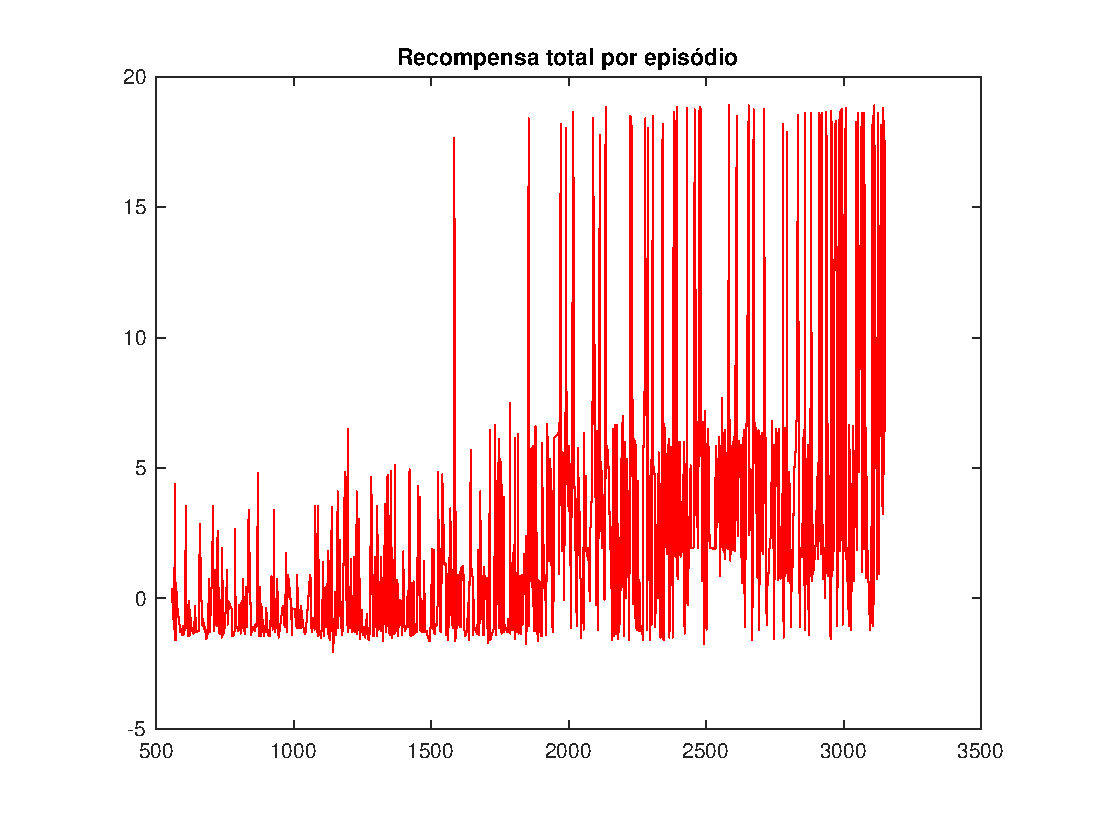
\includegraphics[width=.5 \textwidth]{imgs/resultados/historico_recompensa_v1.eps}
  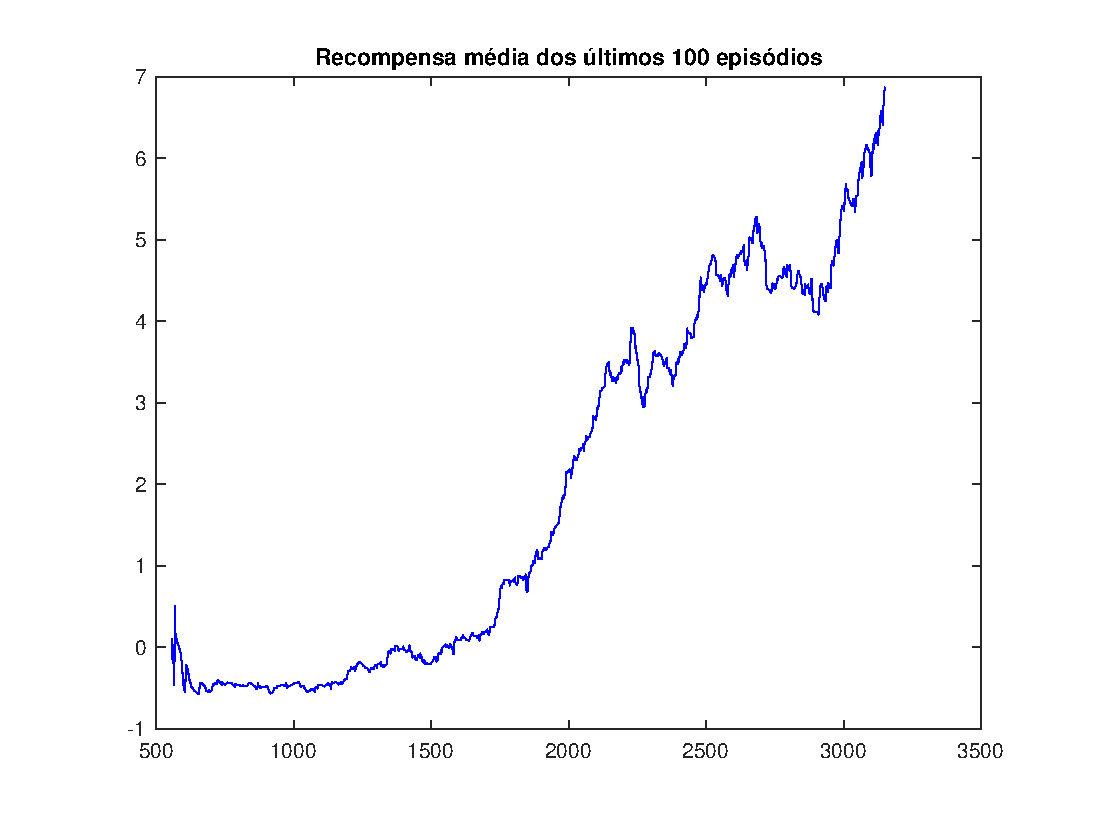
\includegraphics[width=.5 \textwidth]{imgs/resultados/resompensa_media_100_epis_v1.eps}
  \label{fig:resultados_v1}
\end{figure}
\end{frame}

\begin{frame}{Resultados}
	\begin{figure}
		\centering
		\animategraphics[autoplay,loop,width=.6\textwidth]{2}{imgs/gifs/frogger_epi_best_}{1}{12}
	\end{figure}
\end{frame}

\begin{frame}{Resultados}
	\begin{figure}[h]
  \centering
  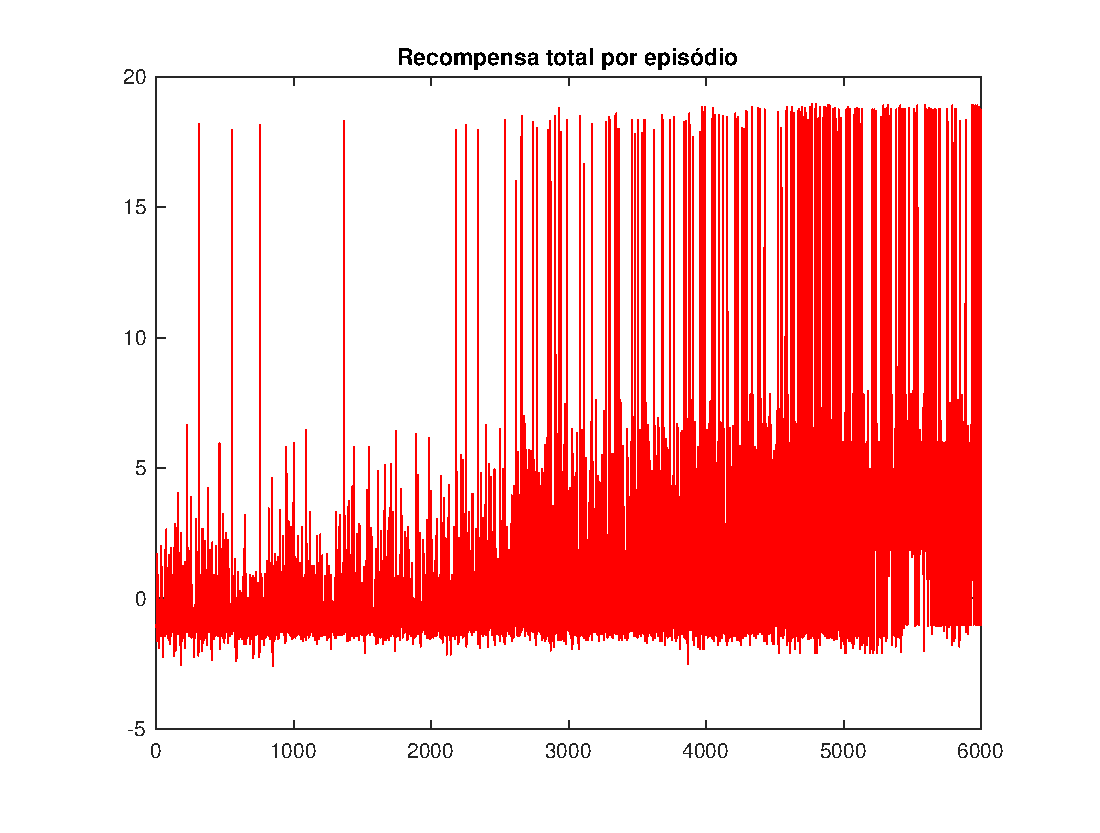
\includegraphics[width=.5 \textwidth]{imgs/resultados/historico_recompensa_v2.eps}
  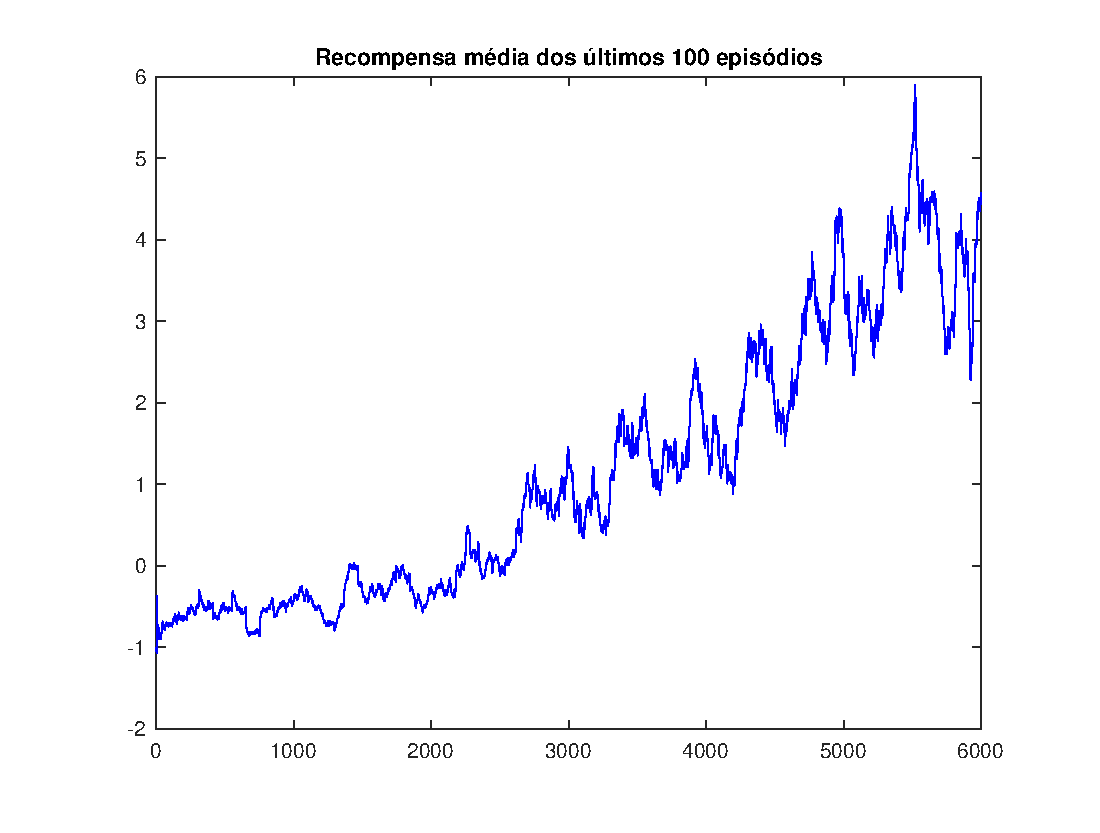
\includegraphics[width=.5 \textwidth]{imgs/resultados/resompensa_media_100_epis_v2.eps}
  \label{fig:resultados_v2}
\end{figure}
\end{frame}

% ----------------- Nova Seção --------------------------------
\section{Considerações Finais}
\stepcounter{subsection}

\begin{frame}{Conclusões}
	\begin{block}{}
		\begin{itemize}
			\item Resultados obtidos são limitados mas promissores
			\item Agente foi capaz de encontrar uma política claramente superior à uma abordagem aleatória
			\item Dado um ambiente de treinamento mais propício, e com tempo de treinamento suficiente, espera-se que o sistema encontre resultados ainda melhores
		\end{itemize}
	\end{block}
	\pause
	\begin{block}{Limitações}
		\begin{itemize}
			\item Comunicação entre o jogo e o ALE é limitado
			\item Aumenta o tempo de processamento dos dados
			\item Uma comunicação direta e em tempo real tornaria possível a implementação de soluções que poderiam otimizar o processo
		\end{itemize}
	\end{block}
\end{frame}

\begin{frame}{Propostas de Continuidade}
	\begin{block}{}
		\begin{itemize}
			\item Executar o sistema em um período suficientemente longo para obter um modelo com uma política equiparável à de um agente humano
			\item Desenvolvimento de uma comunicação direta em tempo real entre o ALE e o jogo
			\begin{itemize}
				\item Cálculo da pontuação poderia ser feita pelo jogo e não pelo ALE
				\item Possível implementação de uma solução que evite a renderização das imagens do jogo
				\item Redução da margem para erros e possibilitando um sistema ainda mais genérico
			\end{itemize}
			\item Aplicar o sistema para outros jogos com diferentes mecânicas de forma a avaliar melhor o potencial da rede implementada

		\end{itemize}
	\end{block}
\end{frame}


% ----------------- NOVO SLIDE --------------------------------
\section{Referências}
\stepcounter{subsection}

% --- O comando \allowframebreaks ---
% Se o conteúdo não se encaixa em um quadro, a opção allowframebreaks instrui 
% beamer para quebrá-lo automaticamente entre dois ou mais quadros,
% mantendo o frametitle do primeiro quadro (dado como argumento) e acrescentando 
% um número romano ou algo parecido na continuação

\begin{frame}[allowframebreaks]{Referências}
\bibliography{referencias}
\end{frame}

% ----------------- FIM DO DOCUMENTO -----------------------------------------
\end{document}
